\documentclass{article}
\usepackage{geometry}
\usepackage{fancyhdr}
\usepackage{amsmath, amsthm, amssymb}
\usepackage{graphicx}
\usepackage{hyperref}
\usepackage{courier}
\usepackage{color}

\title{MLEND Capstone Project: Training a Smartcab Planner}
\author{Lucas Murtinho \\ \url{lucas.murtinho@gmail.com}}
\date{2016-Jul-20}
\begin{document}
\maketitle
\tableofcontents
\newpage

\section{Definition}


\subsection{Project Overview}

In Project 4 of Udacity's Machine Learning Engineer Nanodegree, I had to teach a smartcab in grid-like world how to get to a destination on time by obeying traffic rules and following the directions passed by a planner. Without any kind of hard programming, the agent should learn right-of-way rules and to go straight when the planner sent a "forward" input, for instance.

A natural extension of this project is, instead of relying on an outside planner, coming up with an agent that, given the smartcab's location and destination, learns how to plan a route. This is the goal of my capstone project.


\subsection{Problem Statement}

The problem at hand is to program an agent that learns to identify what the next waypoint should be for a smartcab in a grid-like world to reach its destination as fast as possible. I'll use an $8\times6$ grid for the project, similar to the one used for the Nanodegree Project 4, but in principle the solution should apply to a grid of any size.


\subsection{Metrics}

The goal of the planner is to come up with the best possible action for the smartcab at all times. As we will see, it is not hard to write a planner that always comes up with the best next waypoint (not taking into account eventualities such as red lights or traffic jams). I'll present such a "perfect planner" in the \hyperref[sec:benchmark]{Benchmark section} below. The main metric I'll use to evaluate my learning agent, then, is the \textbf{rate of agreement} with the perfect planner.

However, it is possible that a learning agent will come up with a different action that is just as good, or even better, than a "perfect planner" would. Therefore, I'll also keep track of metrics such as the number of steps needed for the planner to reach the deadline (again disconsidering the possibility of red lights or traffic; i.e., the agent will always be able to move), and also, more generally, the number of destinations reached.

Finally, I'll also keep track of the sum of rewards received by the agent. However, as we'll see in the \hyperref[sec:algos]{Algorithm and Techniques} section below, the rewards are just a means to an end: they exist to get the agent to learn the desired behavior, and its accumulation only matters inasmuch as it helps with this goal.


\section{Analysis}

\subsection{Input Space Description}

In Project 4 of Udacity's Machine Learning nanodegree, the world in which the smartcab existed was represented by a graphical $8\times6$ grid rendered in Pygame. I'll use an image of that world in the \hyperref[sec:explovis]{next section}, but for now I'll describe the problem's input space abstractly.

In the grid-like world of the smartcab, each position is defined by an $(i, j)$ tuple, in which $i$ is the longitude (the position across the East-West axis) and $j$ is the latitude (the position across the North-South axis). In a $m\times n$ grid, $(1, 1)$ represents the northwesternmost position, while $(m, n)$ represents the southeasternmost position.

The goal, then, is that, given a position tuple $(i_{cab}, j_{cab})$, a destination tuple $(i_{dest}, j_{dest})$, and a heading (described below), the planner should be able to come up with the best next action for the smartcab: \texttt{forward}, \texttt{right}, or \texttt{left}. 

The results of an action taken by the smartcab depends on its heading. The heading is a tuple $(i_{head}, j_{head})$, whose items represent East-West heading and North-South heading, respectively. The heading tuple must obey the following rules to be valid:

\begin{enumerate}
   \item The value of a tuple element indicates how the smartcab will move along the element's axis if it moves forward. This value can be either -1, 1, or 0.
   \item If the first element of the tuple is non-zero, the second element is zero and vice-versa. (This means the smartcab can only be headed in one direction at a time.)
\end{enumerate}

These rules imply four valid headings: $\{(1, 0), (-1, 0), (0, 1), (0, -1)\}$. These headings indicate the smartcab is turned East, West, South, and North, respectively.
 
Therefore, if the smartcab is at position $(i_{cab}, j_{cab})$ and moves forward, at the next step it will be at position $(i_{cab} + i_{head}, j_{cab} + j_{head})$ - with an important exception: the grid world is \textit{toroidal}, which means going "over the border" will bring the smartcab to the other side. If the smartcab is headed East at the eastnorthernmost position $(8, 1)$ in an $8\times6$ grid, for instance, moving forward will bring it to the westnorthernmost position $(1, 1)$. 

The more general formula for the smartcab's position at the next step after moving forward (considering, as stated above, that $(1, 1)$ represents the northwesternmost position in an $m\times n$ grid) is therefore:

\begin{equation}
((i_{cab} + i_{head} - 1) \% m + 1, (j_{cab} + j_{head} - 1) \% n + 1)
\end{equation}

The above expression is used to update the smartcab's location in the current version of the environment class used for project 4 (see \href{https://github.com/udacity/machine-learning/blob/2b6a7fca8ea43e00519f426a6b4ad3a130fca737/projects/smartcab/smartcab/environment.py#L195-L19}{here}).

I created the following functions to create the input space for the planner:

\begin{enumerate}
    \item \texttt{get\_delta(location, destination, grid\_size)}: given the smartcab's location, its destination, and the size of the world, this function returns a tuple with the shortest East-West and North-South distances between the smartcab and its destination. If the shortest distance is going East or South, the corresponding element in the returned tuple is positive; if the shortest distance is going West or North, the element is negative. (In other words, delta has the same sign as the heading the agent should be in to take the shortest path to its destination.)
    \item \texttt{get\_distance(delta)}: given a delta tuple, this function returns the Manhattan distance from the smartcab's location to its destination. It will be used to compute the reward the smartcab will receive at each step.
    \item \texttt{get\_next\_point(position, heading, grid\_size, action)}: given the smartcab's position, its heading, the grid size and the action the smartcab is to perform, this function returns two tuples:
    \begin{itemize}
        \item The next position of the smartcab
	\item The next heading of the smartcab
    \end{itemize}
    For instance, if the smartcab is at position $(1, 1)$, facing North, and goes right, its next position will be $(2, 1)$ and its next heading will be to the East.
    \item \texttt{get\_random\_position(grid\_size)}: given a grid size, this function returns a random position in it, considering is northeasternmost position is $(1, 1)$. This function is used to initialize the smartcab's and its destination's positions for a new trial.
    \item \texttt{simulate(trials, grid\_size, deadline, planner\_func, qval\_func)}: given the number of trials, the grid size, a function that defines the planner's action at a given stated and a function that updates the $Q$-values for each state-action pair, this function simulates the smartcab world, in the following way:
    \begin{itemize}
        \item The overall sums of rewards and time left (explained below) are set to zero
	\item For the number of trials defined when calling the function:
	\begin{itemize}
            \item The smartcab's and destination's positions are randomly initialized using \texttt{get\-\_random\-\_position}, and the smartcab's heading is also randomly defined
            \item The delta tuple is calculated using \texttt{get\_delta}
	    \item The state is defined as a tuple containing the delta and the smartcab's heading
	    \item The state and the current $Q$-table are passed to \texttt{planner\_func}, which returns an action
	    \item The smartcab's position and heading are updated using \texttt{get\_next\_point}
            \item The reward associated to the new location is calculated by \texttt{get\_reward} (explained below)
	    \item The previous state, the action performed, the reward perceived and the current state are passed to \texttt{qval\_func}, which updates the $Q$-table
	    \item The reward perceived is added to the overall sum of rewards
	    \item If location is equal to the destination, the difference between the deadline to reach the destination and the number of steps taken by the smartcab since the beginning of the trial is added to the overall sum of time left
	\end{itemize}
    \end{itemize}
\end{enumerate}

\subsection{Exploratory Visualization}
\label{sec:explovis}
Figure 1 shows the grid world of Project 4 without the lights and the other ("dummy") agentes. This is the world in which the planner must find the best route toward the destination.

\begin{figure}
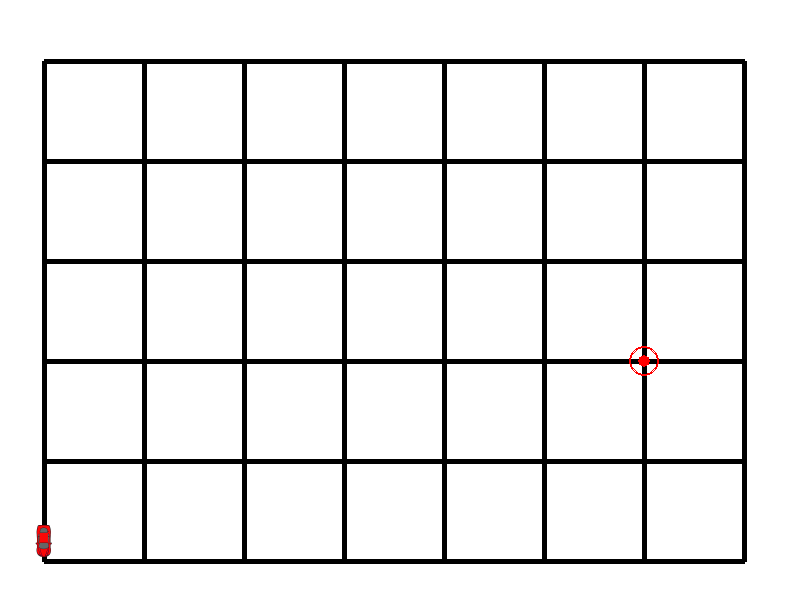
\includegraphics[width=\textwidth]{planner_world}
\centering
\caption{The planner's world. The smartcab is at position $(1, 6)$, facing South, and a forward move would therefore take it to position $(1, 1)$. The destination is at position $(7, 4)$. Due to the toroidal nature of the world, the smartcab's next move should be \textit{right}, taking it to position $(8, 6)$ and 3 moves away from its destination.}
\end{figure}

\subsection{Algorithm and Techniques}
\label{sec:algos}
\textit{Q-learning description}

\subsection{Benchmark}
\label{sec:benchmark}
\textit{Random planner and perfect planner - table results}


\section{Methodology}

\subsection{Data Preprocessing}
\textit{No data preprocessing (but mention transformation of delta into distance)}

\subsection{Implementation}
\textit{Q-learning model (maybe code?) - number of trials and deadline per trial}

\subsection{Refinement}
\textit{messing atround with parameters}

\section{Results}

\subsection{Model Evaluation and Validation}
\textcolor{red}{???}

\subsection{Justification}
\textcolor{red}{???}


\section{Conclusion}

\subsection{Free-Form Visualization}
\textit{boxplot showing results per planner + plot with learning planner result per trial}

\subsection{Reflection}
\textit{Does agent consider if it's easier to turn right or left (or go forward)?}

\subsection{Improvement}
\textit{Improvement: put planner and smartcab together to learn how to play around traffic or red lights}
\textit{Improvement: modify get\_distance code to consider modular arithmetics}
\textit{Modification: what if the grid world is not toroidal?}

\end{document}
